\chapter{Introduction}


%****************************************
% Structure of this chapter
% Section: explain the topic and its significance, raise curiosity, give some facts about it.
% Section: state the the purpose of this study, specify the focus of it.
% Section: overview of chapters and structure of thesis.
% Section: a note on terminology, clarification about the comprehensive terminology.
%........................................


%****************************************
% Sample phrases:
% The discussions (mentioned discussion are also formed the thesis project entitled ... )
% Aim of this thesis is ...
% There has been a recent spate of artistic work focusing on (over-)consumption using the lens of disposal and discard.
% as a reaction to the consumerist society.
%........................................


\epigraph{One can even shout out through refuse \ldots}{\hfill---Kurt Schwitters, \textit{Kurt Schwitters}, 1985}


%****************************************
% Rubbish: the archaeology of garbage. rathje1992rubbish
% Garbage project's findings have supplied a fresh perspective on what we know --- and what we think we know --- about certain aspects of our lives. p.24

% The basic methods of garbage disposal are four: dumping it, burning it, turning it into something that can be useful (recycling), and minimizing the volume of material goods.(p.33)

% ancient peoples p.33

% fast food packaging. p97

% human behavior p.55 can you tell a lot about the customers from their garbage?

%p191-192 people tend to think of "recycling" as a relatively modern conceit that has only recently gained broad public acceptance, and whose practical benefits have only just began to be realized. Recycling itself is probably as old as --- indeed, seems to be a fundamental characteristic of --- human species.

%p.209 The reuse of paper, for example, involves processes that generated a considerable amount of hazardous waste. In order to recycle newspapers, magazines, and, indeed, any printed paper, the paper must first be de-inked. At the end of the de-inking process one is left with essentially two products: on the one hand, de-inked fiber that will be turned into new paper; and on th other, a large quantity of toxic sludge.
%........................................


%****************************************
% trasformations 

% during great depression, I learned firsthand about frugality as a child during ww2. my family carefully folded the wrapping paper from gifts to reuse on other occasions. p.8

% p11. for decades we've taken for granted used cars and old houses. Is there anyone alive who has always lived in new houses or driven only new cars?

% p.11 Economics has always been a factor in recycling. 

% p.12 recycling is not limited to folk art. 

% Bicycle wheel duchamp 1913.

% Use of recycled materials is not new, not is it exclusive to the united states. p.18

% p.22 Material, meaning, and memory --- these are artists' reasons for using found objects.

% p.48 recycling may be the most wasteful activity in modern America --- a waste of time and money, a waste of human and anutral resources. john tierney, "What a Waste," seattle postintelligencer...
%........................................

Common perception to the trash is to get rid of it as soon as possible. People want to depose trash from their lives most of time not thinking beyond. However to establish solid understanding of trash, we have to give attention to the trash and ask why it is trash? How does it become trash? 

\paraphrase{Every day, we put unwanted material in toilets and garbage bins, regularly flushing it away or taking it out in bags to be transported far away from our homes by others. The names we give this material ---waste, garbage, refuse, trash, rubbish--- have pejorative definitions. Worthless. Rejected and useless matter of any kind. Unimportant. Our trash is a testament; what we throw away says much about our values, our habits, and our lives. While dictionary definitions of garbage describe it as “filth” and “worthless,” scholars are careful to note that perceptions of waste and the value of material are neither static nor universally shared. \ldots the question of who owns these discards is not trivial. The absence of a waste stream aroused suspicion, just as the presence of particular items tell us about the habits of the consumers who generate a waste stream. Our trash is part of us, whether or not we choose to acknowledge it \cite{zimring2012encyclopedia}}. \todo{ref for tracey emin et al.}

In this thesis work to understand the different aspects of trash is a key element. \todo[inline]{These aspects are \ldots} As scholars agreed on \todo{ref.} it is part of our life and daily practice and it is very common concepts from developed cities to rural areas, from modern societies to ancient societies. Sometimes it is accepted as a problem (waste crises, ecological problems.) that is need to carefully and seriously managed. On the other hand it is accepted as a source of diversity. (To establish a solid understanding for trash, it is important to see its dilemmas (it is really a dilemma?) or aspects). Therefore we should ask these questions: What is trash? How does it became trash? Is it a end product or a source material? How much is it valuable? How much is it dangerous?

%\comment{In previous ages (which age? pre industrial ages?) objects and resources are used again and again. Production of objects are hard and laborious. Böyle çok fazla kullanılan nesneye örnek bulsak ne kadar güzel olur. Mendillere bunlara örnek olabilir. Aslında tam benim konumla ilgili çünkü tek kullanımlık. Hijyen kavramıyla ilgili giderek artan da bir ilgi necesiyle tek kullanımlık peçeteler gittikçe önem kazanıyor. Peki burda illaha geçmişe falan girmek gerek var mı? çok mu derdimde benim?}

%\comment{Dört bir yanımız metalarla çevrilmş durumda, istediğimiz şeylere çok kolay bir şekilde ulaşabiliyoruz. Yemek siparişi veriyoruz ayağımıza geliyor. İki blok ötedeki kahveciden istediğimiz zaman kahvemizi alıyoruz. Ama tüm bunların bir bedeli var. Bir yandan da sürekli olarak çöp üretiyoruz. Her ne kadar son derece sistemli bir şekilde çöpler toplanıyor ve belki de ne kadar tüketildiğini hiçbir zaman farkına var mıyoruz?}

% Trash is everywhere and, produced every time
Modern (developed) societies are continuously generating trash and, pile them on landfills. During daily activities (drinking, eating, waiting in the bank?) trash is generated and people get rid of them as quickly as possible. (Various objects become trash after their primary functions consumed. People do not care the package of the objects that they buy. They buy the coffee not the cup of it. After coffee finished the life of cup also finishes. Very small life. But is that really so? Is that really life of an object ends after tossed on the waste bin? \todo{Rubbish Theory, Zizek} (Objects life time in the nature is more than human being. People use them for just 5minutes, however they will exist years on the nature.) The vast amount of industrial discarded items spread through the landfills to oceans. They are the result of highly complex industrial production methods. \comment{They are not easily disposable items in the nature.} They live in the nature thousands of years. They are durable(in terms of resistant to natural affects) products. Most of them packages that are used to carry or protect other materials. After real material used these packages became valueless (or useless). (types of trash can be mentioned here, but currently in the artwork I'm using paper packages, therefore, it is more important.) How manage the all this increasing trash that damaging nature?  This is the common approach to trash and the main problem. (actually the sustainability problem.) It is not the only problem, It can be thought that it is a losing the ability to transform new things, alternative behaviors etc. (Instead of creating new opportunities or alternatives, it is a consuming all of them (which?) and producing huge pile of trash.) 

\textbf{Trash is global}, and shared concept for all societies throughout the ages. 
\textbf{Trash in every age.} In other words it is part of human activity of every historic age. It exists early ages of human to now. Trash is part of the early days of human production / or activity. Archaeologist find things from people throw away. 
\textbf{Trash in every society.} Some of them called as trash the others don't. Somehow all actions of people generate trash. It is common. 
\textbf{Trash is everywhere.} in the streets, in your home, in the sea that you swam, around the globe \todo{satellite discard covers the atmosphere}. Even if trash is isolated by people, it is close as closest waste bin.

[RELATIVE] As stated by the editor of Garbage issue of ReVista, Christmas decorations at Chocó, a poor region on Colombia’s Pacific Coast, are \quotes{all crafted from used tin cans, old newspapers, discarded textiles and found wood objects} \cite{erlick2015editorsletter}. She realized that any of them called the practice as recycling. For them using trash again and again is very natural and it is part of their life. On the contrary for the developed countries trash considered as a thing that must be avoided. There is no place for trash in their life. It can be understood that approach to the trash is not same for the all regions of world \todo{ref}.

% FROM Trash as Treasure BY WILLIAM L. FASH AND E. WYLLYS ANDREWS, ReVista
% TODO PRAP.
[FACTS] \paraphrase{The World Bank estimates that the amount of solid waste generated in cities is growing faster than the rate of urbanization. The higher the income level and the rate of urbanization, the greater the amount of solid waste produced. OECD\footnote{OECD(Organization for Economic Co-operation and Development) is an international economic organization of 34 countries. Turkey is member of this organization.} countries produce almost half of the world’s waste. Africa and South Asia produce the least waste. High-income countries have the highest collection rates and are most likely to dispose of waste to landfills or incinerators. Low-income countries have the lowest collection rates and are most likely to dispose of their waste in open dumps. However, low-income countries also have the largest numbers of informal waste pickers who collect, sort, and reclaim recyclables---thus reducing costs to the city and to the environment \cite{fash2015trash}.} \todo{Zengin adamın harcama lüksü}

% FROM Beautiful Trash Art and Transformation BY PAOLA IBARRA, ReVista
% TODO PRAP.
\paraphrase{\textbf{We relate to garbage daily. We use it, produce it and dispose of it. Endlessly. The most obsessive of us get rid of it as fast as we can.} The hoarder likes to salvage a few things for later use---the plastic and glass containers, the cardboard boxes. We know that capitalism’s escalating cycles of production, consumption and obsolescence keep worsening an already problematic relationship between humankind, waste and nature (not to mention social and economic relations). Despite a relatively increased awareness about consumption and its consequences, the pace at which we also acquire and dispose of material objects is exploding. Particularly in the connection between garbage and the arts, \textbf{I am interested in two questions. First, the issue of recycling as a general practice in the arts; and secondly, in the whole issue of representation---that is, representation of waste as subject, and representation (of waste or others subjects) through waste as material} \cite{ibarra2015beautiful}.}

People tend to think that trash is valueless because it is trashed no longer needed or not wanted anymore. However is it really values? What does make it valueless? 

People do not think what happens after they throw it away. It exits from your life but not the world. What happens when you throw it away? It is stacked from another place. Value of objects are not static. Trash is not static \todo{ref. first paragraph.} also it has a long journey. A project conducted by MIT researches journey of trash by placing trackers onto the trash \cite{chen2009mit}. The results are surprising. Trashes spread away across the country and this journey takes month. \todo[inline]{give exact reference} We know that it is not limited with the border of America because it is the one of the countries export their garbage to the other countries --- fourth world countries\todo[inline]{footnote what are these countries?}. In other worlds Americans trash is not only their trash. As commodities spread to the every corner of the world, trash also. What happens when it is traveled to the other countries, how they approaches these items. \comment{They find new uses and meanings on them.} \todo[inline]{consider Papua genen people}

\begin{quote}
\paraphrase{“Nobody wonders where, each day, they carry their load of refuse. Outside the city, surely; but each year the city expands, and the street cleaners have to fall farther back. The bulk of the outflow increases and the piles rise higher, become stratified, extend over a wider perimeter” – Italo Calvino, Invisible Cities} The project is an initial investigation into understanding the 'removal-chain' in urban areas and it represents a type of change that is taking place in cities: a bottom-up approach to managing resources and promoting behavioral change through pervasive technologies. TrashTrack builds on previous work of the SENSEable City Lab in its exploration of how the increasing deployment of sensors and mobile technologies radically transforms how we understand and describe cities. “People just take their trash and put it on the curb and they forget about it and don’t think about all the time and energy and money put into disposing of it.”
\end{quote}

% Cycle of trash
Trash moves, objects moves from place to place. From homes to garbage trucks. From streets to land fills. From garbage baskets to sculptures. \todo[inline]{REF. MIT Garbage project} Lots of different people touches to trash. With the trash what moves?

% ARTWORK http://timgaudreau.com/2012/trash/trash.html
[ARTWORK] \comment{Self-Portrait as Revealed by Trash} Even if people pay little attention, everybody do not. An artist takes photos of his every trash, like people take photos of their faces. He focuses on the thing that paid little attention, that is trash. At the end he exhibits all the photos by covering all the walls of room. It can seen as record of his activities, record of commodities. Most of them we are not aware of them. Draw the attention of is being thrown away and every time and everywhere. They are too much and can only fit covering all the walls. \todo[inline]{Tim Gaudreau “Self-Portrait as Revealed by Trash: 365 days of photographing everything I threw out – Variation I, 2006”} \paraphrase{After photographing my trash over the course of the year, I ended up with 5,000 images representing my waste stream. These collections of grids represent my first experiments with using those images. This initial work ultimately led to the full scale collages that have become my Self-portrait as Revealed by Trash: 365 days of photographing everything I threw out.}

% ARTWORK http://www.keaggy.com/chairs/sad/12/
\todo[inline]{Sad chair. Photos of lonely chairs that are no longer wanted. Artist captures the continuously left alone chairs.}

Why people are interested in rubbish. Some of the artist also interested in others trash. \comment{O çöplerde ne bulmayı umuyorlar ki? Aslında çöp bizim davranışlarımız, yaşayız tarzımız hakkında bize yön veriyor. ve bu her zaman fiziksel dönüştürme ile değil de aynı zamanda anlamsal ve mekansal değiştirme sorulamalarla mümkün oluyor. Bazen de olduğu gibi kullanıyorlar. bu açıdan önemli. Çöpü çöp şekliden sunan sanatçılar. Ama bu nasıl mümkün ki? fotoğrafını çekenler aslında gerçekten ona müdahele etmemiş mi oluyorlar. Bence değil? bir şekilde müdahele var gene orada. o fotoğraflarda artık dikkatin objesi haline geliyor. çöpün dönüşmesi aslında bir diğer yandan çöpe bakışın değişmesi olarak görülebilir.}

% TODO Life time of objects.
% Nesnelerin yaşam süreleri... Can you imagine how much plastic cup is being consumed every hour?

% Şöyle bir şey var, sanata non-art objelerin girmesinden bahsediyoruz ama artık orda o seviyede değiliz. O zamandan bu zamana çok şey değişti. 
\comment{In the beginning of the 20th century non-art objects enter the scope of art making. This is a revolutionary change in the making of art. Production of art and the approach to the art changed dramatically. This changes actually started at the end of the 19th century with impressionist. (But not related with non-art objects.) Picasso is the first artist that used non-art object in his works. Later many of them followed him. First works are collage which gluing different papers together. Yes using non art objects in the art is introduced and opened new dimensions for the language of art. But some of them treated as sculptures from trash. Reflects our world. But it is not limited with this. Some of the works are provokes the consumption habits of society and offers an alternative perception.}

This trash phenomena catches the attention of artist. It is very human activity. In this context which trash? What type of discard. Human discard. trashes of human activity. items that belongs to human. commodities etc. 

%****************************************
% EVERYTHING CAN BE TRASH. Act of trashing not act of transforming. Trash is like kara delik gibi ışığın odan kaçamaması gibi hiç bir şeyin ondan kaçılmayacağını hissediyor aslında. 
% Michael Landy's Art Bin uses a art gallery to create his dust bin. Describing the work, simply called Art Bin, as 'about failure', Landy is inviting members of the public to bring their own artistic failures along to the gallery from 29 January, where their worthlessness will be assessed. Damien Hirst, Gillian Wearing, Tracey Emin and Mark Titchner have already contributed, offering sculptures, paintings and prints. "There's no hierarchy once they are in the bin" All of them are accepted as same. Ultimate equality. Tosing them to the dust bin makes them rubbish even if they are combined from failed attempts. Nothing's too good for the art bin. Everything can fit into the art bin. Michael Landy transforms the SLG into Art Bin, a container for the disposal of works of art. As people discard their art works the enormous 600m³ bin becomes, in Michael Landy’s words, “a monument to creative failure”. It is a very big glass bin and isolates people. There is a provocative approach to the art and art objects by saying that "Nothing's too good for the art bin". There is no limitation of throwing away even if art. 

% Herkes çöpü dönüştürmüyor, bazıları ise çöpe dönüştürüyor. Ama ben bununla ilgilenmiyorum aslında.
%........................................

\todo[inline]{ArtBin, squeezing. [Trashing Things, Artwork]}

%http://www.smithsonianmag.com/arts-culture/photographer-creates-fine-art-out-trash-we-throw-environment-180951615/?no-ist
\todo[inline]{showing trash as they are... [Artwork] by Barry Rosenthal}

%****************************************
% Different types of trash
\todo[inline]{Different types of trash.} \comment{There are many works from trash around the world. Build up trash. Collected from graveyards, landfills, unused materials etc.}

The complexity of produced trashes of societies is increasing. For example developed countries that have nuclear plant generates radioactive wastes which highly hazardous for the environment is never exist previous societies. Think batteries and so on. Every society generates different types of wastes. Differs from country to country, society to society, ages to ages. It can be thought that when the complexity of trashed increased required effort to repair, reuse and recycle is also increase. Therefore for the ones that have no complex tools it is becoming harder to reuse objects. In other words objects become more complex their re-usage becomes less likely.  Different production process generates different types of trash. According to production process, decomposition process\ldots The approach to the different type of trash will be different. In other word if trash is a result of classification of objects, it can be easily extracted that there is classification inside of it. There are some trashes that are more close to the people. More easy to convert them. more easy to regain to the society. 
%........................................


%****************************************
% Different disciplines, Perspectives related with trash from different disciplines
\todo[inline]{List of disciplines, and their approach to the trash.} \comment{Trash draws attention different peoples and disciplines. In other words there are different studies related with trash. Different approaches to the trash and son on.}

% From Trashion: The Return of Disposed, Bahar Emgin.
\paraphrase{Such a conceptualization of waste as “the degree zero of value” has been contested for some time in different disciplines, ranging from economics to environmental studies, but most particularly by those studying consumerism or material culture.}

This is very important because the problem of trash is being tried to be handled by different disciplines. In other words there different approaches to the trash. Different problems, different solutions. Which perspective that I have. In what ways my project differs from them. The purpose is to participate people in this work, by collecting them etc. And also offer to transform it. Rescue it and than later transform it. In short, the difference between the other disciplines must be clear. 
\begin{itemize}
\item Ecological perspective: Trash causes ecological problems and it treats the balance of nature. Animals do not aware of plastics materials and they unconsciously eat them.
\item Management of it (handled by the municipals generally).
\item Technological perspectives. (seeing trash as a design problem. developed technologies and societies generates lots of trash, so this situation cause to inquiry that are they really developed? development in what sense?)
\end{itemize}

\comment{Trash draws attention of many scholars and people who are professional in different areas. Further trash is a common subject of the all ages through the human history. In other words this topic is not introduced in recent years (or ages). It always part of the human practice and life. Even if trash is refused and discarded thing, there are people giving attention to them.}
%........................................


%%%
%%%
%%%
\section{Purpose of the Study}
\todo[inline]{what do you mean when saying ``transforming trash"? Needs to be opened. I claimed that such a thing exist? when it is exist? by physically or conceptually? actually both of them exist.}

The aim of this study is to explore the theories and methods in transformation of trash in the context of art and artistic act.

In this thesis (re-)usage of discarded materials in the process of art making and the artwork itself is explored. Why and how are they used by the artist? Are there any differences with the original items compared to discarded items? Has using discarded material or trash specific (or special) meaning and message? This is a work to explore the re-usage of trash in artworks (place or the role in the art practice). (and also in which scope? medium, message, life practice\ldots) 

As many people are inside the business of transforming trash through craft and so on. People on the streets looking for aluminum cans, glass bottles, plastic. They collect and sell them to survive. There are companies that are collect waste materials to regain them again the industry. In thesis they are not in the scope. People that give attention to the trash and behave artistic act is in the scope of this thesis.

\comment{How does it become trash?} Here the purpose is to understand the dynamics that turn objects to trash. By understanding them is provide a road map (or ideas) how to turn trash to something valuable? (The purpose of this thesis is to find (or explore) a way(methodology, approach) to add value to object using artistic methods? Therefore first question is why they are less-valued, and ignored. How to make them valuable? How to make them part of our life again?)

%%%
%%%
%%% 
\section{Structure of the Study}
This study is structured by many examples of artworks in different part of the thesis. When a topic or argument is presented, immediately example artwork is given at this moment and how artist replies this issue is illustrated. Thereby artworks are examined in the theoretical and cultural context. Artworks are used as a supportive elements for the stated arguments.  However, not every time artworks are discussed in detail. Only basic information is given and how it is related with this topic explained. \comment{By the way} it is better to keep in mind that all works can be analyzed in different contexts in more detail fashion.

Following chapter, Trash in Culture and Theory, explores the place of trash in the cultural life and theoretical approaches on trash. The aim is (better) to understand the trash in cultural and theoretical aspects. (to better realization the notion of trash.) Provides theoretical and cultural background. It is explored the trash is being worked is whose trash. Or what type of society generate this trash. Also in the project I collect the paper trash. What type of approach generate it and what are the dynamics of it? What type of trash we are talking about? It is understood through the patters of consumption patterns. And to reflect this cultural phenomena what philosophers and scholars say. Artist how they are reflected this notion.and also looked how scholars are conceptualized trash and its movement on the different values system. How explained the transient nature of trash?

Third chapter, Trash (in) Art, seeks the root of using discarded materials in the artworks and looks through the sample artworks and artists. As already artworks are mentioned in the different part of the thesis, in this chapter some of them analyzed deeply. Artists methods and approaches to the subject are stated.

\comment{Fourth chapter consists of the overview of the project. Stated the approach to topic clearly. Development process of the work is presented in detail. I will start with the development process of the work. I believe that the way an artist works and the obstacles that she encounters have a huge impact on how the final work is embodied. Development process of my work shaped the way I think on the subject of my thesis. Therefore, I will explain my process as detailed as possible. Then, I will continue with different aspects of my work; formal decisions and usage of light that I believe carry my work to another level. At the end of this chapter, we will see how my work functions and what it proposes on the image and word relationship.}

\comment{Finally last chapter is reserved for an overall conclusion of this thesis and further suggestions on the subject and the project.}

%%%
%%%
%%%
\section{A Note on Terminology}
Within the scope of thesis only words that are English is examined but in different languages and cultures there might be different naming for various stages of object and trash. Analysis of them may be subject of another thesis. (Garbage, trash, rubbish, debris, detritus, waste, scrap, junk, refuse, discard, disposal, litter: during my research scholars and authors have different names for the stuff.) I realized that many scholars and resources have used different words (or terminology) to define trash. Although there are slight differences between these words, sometimes they are used to signify same concept (or used with same purposes). Understanding diverse vocabulary of this topic before dive into the theory makes more clearer the borders of the work. There is no consensus on terminology. Some scholars uses junk art, others recycling art. The origin of vocabulary of this topic reveals a whole side of human activity: our history revealed by what we have thrown away through the ages. What were people throwing out when these words were coined? From the rubbish: the archeology of garbage gives clearer definition of some these words:

% FROM Rubbish! The Archaeology of Garbage, p.9, rathje1992rubbish
\begin{quote}
Several words for the things we throw away---"garbage", "trash", "refuse", "rubbish"--- are used synonymously in causal speech but in fact have different meanings. \textit{Trash} refers specifically to discards that are at least theoretically "dry"---newspapers, boxes, cans, and so on. \textit{Garbage} refers technically to wet discards--- food remains, yard waste, and offal. Refuse is an inclusive term for both the wet discards and the dry. Rubbish is even more inclusive: It refers to all refuse plus construction and demolition debris. The distinction between wet and dry garbage was important in the days when cities slopped garbage to pigs, and needed to have the wet material separated from the dry; it eventually became irrelevant, but may see a revival if the idea of composting food and yard waste catches on. We will frequently use "garbage" in this book to refer to the totality of human discards because it is the word used naturally in ordinary speech. The word is etymologically obscure, though it probably derives from Anglo-French, and its earliest associations have to do with working in the kitchen.
\end{quote}

Some notes on methods: 

%****************************************
% Reuse and Recycle
One of the most encountered words in this topic (transforming trash) is reuse and recycle. Both of them are used widely by scholars \todo{ref}

According to the dictionary, the word “reuse” means “to employ for some purpose” or “to put into service.” Reusing involves usage of the same product unchanged in form. Reusing lengthens the life of the item or material. Other examples are; buying some items and then selling them as used items, repairing some lawn equipment and reusing them, upgrading a computer, renting books, journals, periodicals, DVDs and others. The main purpose is to make the item last as long as it can. To reuse is to use something again instead of throwing it away or sending it off to a recycling company. \textbf{Why throw something away when you can give it another life?} Reusing is significant way to conserve and be earth-friendly because it keeps items out of landfills and reduces the greenhouse emissions caused by purchasing a new product. Using something multiple times -- like using a disposable container more than once -- is not the only way to reuse; you can also give old items a new purpose. For example, use an empty coffee can to store small craft supplies or an old loofah as a scouring sponge for cleaning sinks.

According to the dictionary, “recycle” means “to treat or process (used or waste materials) so as to make suitable for reuse.” In recycling an item, it is processed into a totally new product. It is an energy consuming process. For example, if we put some plastic bottles, paper, or aluminum items in a recycling bin, these materials may be recycled into a totally different thing as clothing items, fabric, or maybe a quilt. In this process, energy is required which depends upon the stages of transformation.

Recycling occurs when waste in an unchanged chemical form is used in the same process that created the original product. Examples are crushed glass containers (cullet) used to make new glass containers, and scrap metal used in foundries. 

Reusing is possible with re seeing (rethinking). Reusing is possible meet the needs of the human itself. Using creativity and personal approach can change objects functions. It is possible to use objects for different purposes. 

Recycling can be viewed as down-cycling. The object smashed to the small particles to be used later in the production of something else. Although reuse can be viewed as up-cycling that gives another (or more) value to the discarded products. Down-cycling does not generates new meanings it tries to convert the product to already known state to process. 

Recycling is very similar the rotting (decaying), reuse is something like dry tree branches used by birds for their nest. These are two agents of nature to regain their resources.

Many scholar used the word recycling when mentioning works use trash and the concept of it. However they are not mentioning the meaning that is decomposing things to the their particles. What they is actually is reusing and combining things, concepts, creating new mixtures.

It is hard to say that they use it wrongly, but what they refer is actually upcycling. Creative reuse, inventing new things from discard.

% I prefer to use the word waste to describe the things that have, for whatever reason, been leftover from use or for which use has been precluded.

\begin{figure}[h!]
  \centering
  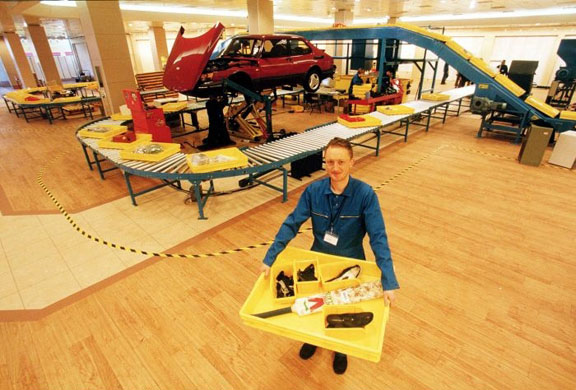
\includegraphics[height=6cm]{graphics/ChrisJordan_BreakDown.jpg}
  \caption{Chris Jordan, Break Down}
  \label{fig:ChrisJordan_BreakDown}
\end{figure}

\paraphrase{Not all artist transform trash although some deconstruct them. Michael Landy is one of them. Michael Landy's Break Down Inventory is a two week show / display of destruction process of his all possessions on a dissemble line with the help of 10 workers. Firstly they are classified and recorded for three years and the deconstructed in two weeks by separating every element to the smallest part. Reveal all his possessions. and loosing them while you are alive. Turning them to rubbish making them unusable. breaking down the all the meaning. breaking down the connections.} It can be an example of downcycling process. It is preferred to decompose all the complex link and relationships between the objects. They are not just ordinary things they are possessions of artist. Break Down 2001, in which he systematically destroyed all his personal possessions. His work examines what we value and what we discard, consumerism and waste, and human labour and its worth. It happens in public space. People can see the process. This process last 2 weeks. Places where people buy things actually.

\comment{Yıktığı şeyler aslında bir noktada hepimizin yaşayacağı şeyler. Bunu yaşarken yapıyor. Tüm sahip olduklarını yaşarken kendi isteği ile bunların hepsini yok ediyor.}

In this thesis scope mainly single use, disposable objects are considered generally. Nearly half of the material used in the project is disposable packets. Therefore as well as other words used but mainly trash is used to refer the material. 

Some of the scholar uses recycling\cite{cerny1996recycled,herman1998trashformations} for the recreation and transformation of it. Some of the scholars and artist uses upcycling for their process. 

%****************************************
% UPCYCLING:
% Burada da upcycling kullanıyor aslında. http://www.gwynethleech.com/cups/suspended
% Raw+Matrial=Art burda da upcycling deniliyor.
%
% RECYCLING:
% recycled, re-seen book.
%........................................
